% !TeX root = main.tex

\chapter{Long Short Term Memory}
Objectif principal de ce projet, l'architecture neuronale Long Short Term Memory
(LSTM) est décrite dans cette partie. Tout comme les autres architectures
neuronales, elle est constituée d'un assemblage de blocs élémentaires qui
disposent d'un ensemble de variables, appelés poids, à adapter lors de la phase
d'apprentissage afin de reproduire une fonction. Cependant, la cellule
élémentaire d'un réseau LSTM est bien plus complexe que celle d'un réseau
neuronal à perceptrons. \\

La dénomination LSTM vient du fait que ce type de réseau possède une mémoire de
plus longue durée que des structures de type RTRL. Ainsi, il sera possible
d'apprendre des fonctions telles que la grammaire de Reber double, ou bien de
générer du texte après avoir appris des écrits de Shakespeare. \\
LSTM est notamment utilisé dans des applications de reconnaissance vocale.

\section{Théorie}
\subsection{Cellule LSTM}
La cellule LSTM est un petit réseau de perceptrons récurrent présentant des
élément nommés en fonction de leur rôle dans la cellule.

\begin{figure}[!ht]
\begin{center}
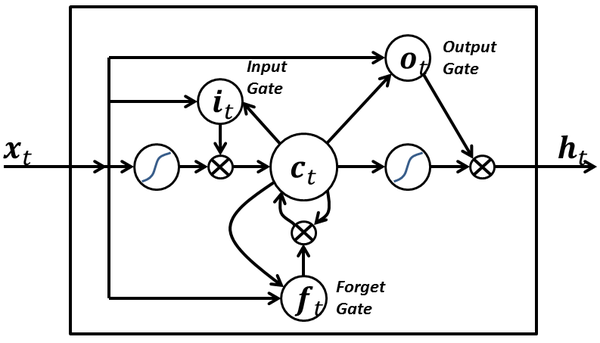
\includegraphics[scale=0.8]{images/lstm.png}
\end{center}
\caption{Cellule LSTM}
\end{figure}

\subsection{Propagation}

\subsection{Algorithmes d'apprentissage}
L'algorithme d'apprentissage est un algorithme BPTT appliqué aux cellules
LSTM considérées.

\begin{figure}[!ht]
\begin{center}
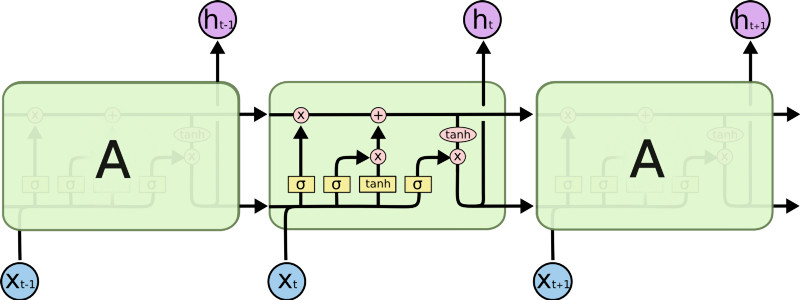
\includegraphics[scale=0.4]{images/lstm-bptt.png}
\end{center}
\caption{Dépliement du temps dans l'espace style BPTT}
\end{figure}

\section{Implémentation}

\section{Résultats}
\subsection{Apprentissage sur un mot}
\subsection{Grammaire de Reber simple}
\subsection{Grammaire de Reber double}
